\newcommand{\MainPrimary}{1792}
\newcommand{\MainAuxiliary}{896}
\newcommand{\MainFresh}{16}
\newcommand{\MainCells}{4}
\newcommand{\MainGroups}{3}
\newcommand{\MainConditions}{16}
\newcommand{\MainDerived}{8}
\newcommand{\CompiledFaultFail}{12}
\newcommand{\DeclaredFaults}{12}
\newcommand{\ControlFail}{0}
\newcommand{\NumericControls}{4}
\newcommand{\OracleDisagreements}{0}
\newcommand{\CompiledWitnessCalls}{16}
\newcommand{\PointwiseWitnessCalls}{12}
\newcommand{\StrongWitnessCalls}{12}
\newcommand{\ParentWall}{234.15}
\newcommand{\NativeCPU}{137.34}

\begin{abstract}
Robot-policy deployment checks answer different questions about an executable interface: whether artifacts match, a decoder preserves an intended numerical map, a transport accepts an array, or sufficient evidence grounds physical meaning. We study these distinctions using pinned native processors and independently constructed references, retaining explicit unknowns. A protocol committed before selected native execution fixes three published metadata groups, four execution cells, sixteen deployment conditions, eight derived authority views and eight query geometries. The acquisition executes \MainPrimary{} primary decoder calls, \MainAuxiliary{} auxiliary round-trip calls and \MainFresh{} fresh witness calls across LeRobot and OpenPI. Compiled affine obligations, independent pointwise checks and a strong relational oracle agree on the full-reference main conditions. With offset authority erased, the two relational methods retain slope detection while the pointwise method abstains. Applicable static statistics and independently referenced round trips match the finite detection counts. Native self round trips remain consistent under changed mappings, while physical authority remains unknown. The compiler's witnesses use more calls than the independent oracles. Separately labeled historical incidents and software-controller experiments clarify temporal and nonlinear scope. The resulting artifact provides a reproducible comparison of evidence requirements and negative findings; it establishes neither detector superiority nor policy competence or hardware safety.
\end{abstract}

\section{Introduction}
An action vector does not identify a complete robot-policy interface. Its interpretation also depends on normalization statistics, coordinate identity, units, action modes and the state against which queued actions are interpreted. A processor can execute successfully while implementing a different map from the one intended by a deployment. Conversely, a checker can correctly withhold certification because essential evidence is absent even when the numerical map agrees on every observed input.

Executable-policy specifications already articulate this problem. In particular, \citet{tai2026execspec} formalizes executable-policy identity and derives normalization-mismatch certificates. Shared policy interfaces and isolated execution environments are also established infrastructure \citep{xpolicylab2026}. We therefore investigate an empirical question rather than propose these concepts as new: \emph{what conclusions survive when different applicable checks receive the same available artifacts and observations, and which conclusions require evidence that public metadata does not supply?}

We develop an executable workflow around explicit, partially grounded contracts. In a source-justified affine fragment, bounded interventions expose coefficients and offsets. An independently implemented pointwise oracle and a stronger relational oracle receive the same observations and reference. Native tools retain their own scopes and verdict vocabulary. File identities, requests, loaded statistics, raw responses and reduced witnesses remain replayable. The workflow also has temporal contracts, but the selected metadata evaluation is action-only; temporal results remain a separate retrospective stratum.

The main evaluation has three artifact groups labeled ACT, SmolVLA and PI05 by their published configuration metadata. LeRobot executes all three; the same PI statistics are explicitly transported into OpenPI. No trained policy is constructed. Four source-derived deployment conditions per cell comprise one intended numerical control and three declared interventions. Two additional views erase authority or units without creating new executions. The study is outcome-unseen at these selected revisions before native acquisition, but metadata inspection, intervention recipes and shared ancestry are disclosed.

Our contributions are an inspectable comparison protocol and artifact, a conditional account of what the admitted observations identify, and an empirical separation of numerical conformance, artifact identity, certification and transport. The main finding is parity: no detection advantage emerges over strong applicable alternatives. The compiler's local witnesses are larger under the measured call count. Missing physical authority persists across every selected cell. These negative findings suggest practical reporting requirements: specify the tested boundary, disclose evidence dependencies, retain inconclusive outcomes, and compare against an oracle that can use the same relations. Automation and auditability are implemented properties; a reduction in human effort has not been measured.

\section{Related work and attribution}
\paragraph{Executable robot-policy interfaces.}
\citet{tai2026execspec} treats weights as one component of executable policy identity and develops model-free normalization drift certificates. We implement its stated finite arithmetic separately from extensions for the pinned framework conventions. Designed processor queries are not demonstration calibration and do not reproduce that paper's simulator outcomes. Its controller-level distinctions additionally require affected outputs on model support and a controller distinction; our probes do not establish those conditions. XPolicyLab supplies policy adapters, schema conventions and isolated runtime/lifecycle infrastructure \citep{xpolicylab2026}. We do not claim these mechanisms as new or infer missing checks from an unexecuted adapter.

\paragraph{Testing and identification.}
Automated metamorphic oracles for action policies predate this work \citep{eisenhut2023}. That setting assesses policy quality with state simulation and cost relations; ours concerns processor meaning under an independent interface reference. CRADLE and EAGLE establish differential backend and equivalent-computation testing for ML libraries \citep{pham2019cradle,wang2022eagle}. Cross-implementation agreement supplies useful regression evidence, but cannot supply an absent physical specification. Model-based conformance has established transition-system foundations \citep{tretmans2008}. Our finite probes do not inherit an ioco soundness result. Failure-preserving reduction is also established \citep{zeller2002simplifying}; the exported local relation witnesses are not globally minimal causal explanations. Three-valued finite-trace monitoring provides a distinct precedent \citep{bauer2011runtime}: temporal-prefix inconclusiveness is different from missing-authority \UNKNOWN{}.

\paragraph{Available tooling.}
We inspect pinned source revisions and execute applicable stock paths in Robotruth, Policy Space, Robot Policy Preflight and ActionABI \citep{robotruth2026,policyspace2026,preflight2026,actionabi2026}. Robotruth's manifests and severity-based unknown handling, and ActionABI's partial-evidence equivalence sets and separating probes, overlap substantially with the conceptual proposal. Policy Space's supported custom registry permits an applicable raw-vector transport comparison even when a stock physical embodiment mapping is unavailable. Tether's full workflow requires paired native/export rollouts and outcome/resource channels \citep{tether2026}. We lack those channels and record that workflow as unavailable, rather than assign it a miss. Publisher performance claims are not reproduced by source inspection or our narrower module executions.

\section{Contracts, observations and conditional identification}
\subsection{Evidence and decision scope}
A contract separates intended numerical coefficients, artifact provenance, coordinate identities and units, physical/controller authority, admitted operator class and lifecycle obligations. Authority is supplied independently of deployment responses. Main-study references decode the pinned metadata with a separate bounded parser and explicit current-runtime formulas; they do not establish the checkpoint's historical training runtime or physical calibration. Physical authority can therefore remain unknown while a raw-index numerical obligation is decidable.

An execution record binds a contract and artifact to reset, observation, chunk creation and dequeue events, when these events exist in the supported adapter. A chunk retains its episode, originating observation and position. For the action-only study, the observed boundary is a native decoder evaluated on explicit numerical outputs supplied in place of learned inference. We do not infer reachable policy outputs, task success or robot commands from this substitution.

Each grounded obligation receives \PASS{}, \FAIL{} or \UNKNOWN{}. A grounded violation takes precedence over incomplete unrelated obligations; otherwise missing required authority, units, observations or coverage withholds a complete \PASS{}. Unknown coefficients remain unknown. Artifact identity, transport acceptance and another tool's native severity aggregate are separate fields. Their results cannot be converted into a common accuracy score without changing the question being answered.

\subsection{Admitted affine fragment}
Within reviewed deterministic compositions of named permutations, affine normalizers, scalar masks and additive anchors, write
\begin{equation}
 u = A z + Bq_{\mathrm{origin}} + Cq_{\mathrm{current}} + b.
 \label{eq:boundary}
\end{equation}
Independent coordinate bounds define normalized coordinates $x\in[-1,1]^n$ and an equivalent map $u=Mx+c$. For the action-only cells, only the action port is present. For queued temporal captures, a worker must reset each trial, create the chunk at the controlled origin and dequeue against the controlled current observation. An algebraic query plan alone does not prove that schedule executed.

The canonical design uses $x=0$ and $x=\pm e_j$ for each coordinate, giving $2n+1$ queries. In exact arithmetic,
\begin{equation}
 c=u(0),\qquad M_{:j}=\frac{u(e_j)-u(-e_j)}{2},\qquad
 \frac{u(e_j)+u(-e_j)}{2}=u(0).
 \label{eq:contrast}
\end{equation}
The last relation checks sampled closure. Paired effects cancel an unspecified offset, allowing a known slope violation to be exposed when absolute offset authority is absent. A manually written relational oracle can use exactly the same information.

\begin{proposition}[Conditional affine identification]
Let the executed implementation and independent reference belong to an admitted deterministic affine class on the same $n$ coordinates, with fixed statistics and a controlled execution schedule. In exact arithmetic, if their outputs agree on a design whose augmented coordinate matrix has rank $n+1$, they agree as affine maps on that coordinate domain.
\end{proposition}
\begin{proof}
For each output coordinate the map difference has coefficient vector $d\in\mathbb{R}^{n+1}$. Agreement gives $Xd=0$. Full column rank implies $d=0$. This is elementary linear algebra, not a new identification theorem.
\end{proof}

Finite matching does not prove class membership: an arbitrary nonlinear map can agree at every query and differ elsewhere. Rotations, clipping branches, opaque callbacks, learned inference and gripper integration are excluded from the affine claim unless independently handled. A source-reading mistake can also make the producer and reference agree incorrectly.

\subsection{Finite precision and witnesses}
The evaluator binds query identifiers to actual executed coordinates, rejects collapsed bounds, checks rank, and retains a binary64 output-resolution diagnostic. General query geometries use exact binary-rational executed coordinates for cancellation. An unknown contribution cancels only when its actual weight is exactly zero. For a selected nonsingular basis and an explicitly assumed measurement model $y=X\theta+e$, $|e_q|\leq\epsilon_q$, a component interval has radius
\begin{equation}
 R_j=\sum_q |(X^{-1})_{jq}|\epsilon_q.
\end{equation}
Passing requires the whole component interval inside its independent tolerance; disjoint intervals fail and overlap remains unknown. Poor observability can therefore withhold full-map conclusions despite structural rank. The numeric allowances used here are empirical development choices, fixed before evaluation; they do not bound arbitrary upstream arithmetic, sensor error or unknown dtypes.

For canonical center/pair/midpoint obligations, a failed offset relation has a one-query witness, a coefficient contrast two queries and sampled closure up to three. General interpolation component intervals can depend on all $n+1$ basis queries. The fresh witness comparison below uses canonical obligations. These sizes concern the local relation, not an entire causal trajectory. Temporal queries can require multiple native actions. Fresh witness processes load the same artifact and execute only retained original queries. Verification requires the same original failed relation and values within the frozen numerical allowances, rather than accepting any subsequent failure.

\section{Implementation and experimental protocol}
\subsection{API, provenance and execution controls}
The Python package provides versioned contract/report formats, a checker, an opt-in \texttt{mltools probe} API/CLI, offline replay, diagnostics and regression exports. Supported contract fields cover camera identity, joint order/units, normalization artifacts, action modes, explicit gripper conventions, chunk anchors, queues and reset. The original checker operates on its supported scalar command model; incompatible end-effector coordinates are not forced into that model. Optional workers isolate framework imports and use CPU profiles. The core replay path requires neither ML framework.

The complete protocol was committed and pushed as \texttt{7513755e9627098c3529c46b3ae9a056d76434a5} before selected native acquisition. It protects 406 source, configuration, input, test and development-evidence files. Each native worker checks those bytes against the immutable commit before imports and after execution. Immutable start records, exact phase prefixes and exclusive claims prevent a saved request from reacquiring a phase. One original output and one clean-reproduction output are declared. Failures retain completed phases and partial timeout streams; prospective retries or tuning require a disclosed amendment. No prospective retry occurred.

Python audit hooks deny observed connection, DNS, bind and listen operations. A source-identified import-time urllib3 IPv6 capability bind remains denied and is recorded separately. These hooks are not an operating-system sandbox. Hashes and trace records are trusted-producer assertions, not cryptographic execution attestation. No live robot, policy weight, paid compute or native execution download is used.

\subsection{Artifacts, roles and experimental units}
The selected metadata consists of ACT boccia, SmolVLA orange and PI05/LIBERO source artifacts with pinned repository revisions and publisher Apache-2.0 declarations. Native LeRobot decoders execute each artifact's explicit current-runtime normalization profile. The fourth cell transports the same PI quantiles into pinned OpenPI processors. It is nested in the PI artifact group and supplies no native OpenPI checkpoint identity. Original unresolved GCS assets are excluded. Appendix~\ref{app:artifacts} lists identities and reproduction entry points.

Each cell has an intended numerical control, an offset intervention, a slope intervention and a fixed composition of the two. These are declared artifact interventions, not newly discovered deployment incidents. Appendix~\ref{app:recipes} specifies their coordinate selection, magnitudes and probe domain. Two derived views erase reference authority or output units while reusing observations. All intervention definitions, exact derivative files and query designs precede the freeze. Development uses a reused ACT lineage and an explicitly authored known OpenPI fixture; neither is relabeled selected evidence. Historical failures and the Panda software-controller stratum remain separately labeled development/retrospective evidence.

The four cells comprise \MainGroups{} published artifact groups, \MainConditions{} actual deployments and \MainDerived{} derived views. They are dependency-linked descriptive units. Shared SmolVLA base ancestry and LIBERO corpus links, metadata inspection and known recipes preclude blinding, ancestry-disjoint or unseen-root-cause claims. Queries, mutations, seeds, the PI transport and clean reruns are repeated measurements. We report counts and equal-artifact-weight leave-one-out sensitivity, without population confidence intervals or mutation-level significance tests.

\subsection{Matched methods, ablations and budgets}
The compiler, independently implemented pointwise oracle and strong pointwise/pair/midpoint oracle receive the same canonical observations and independent reference. Canonical, manual-axis, random-axis and random-dense designs each receive $2n+1$ genuine native queries per condition; random designs use seeds 7, 23 and 101 and a shared geometry evaluator. Static statistics checks independently decode intended/deployed numbers. Real native self round trips and independently referenced encode/decode paths are acquired, rather than inferred algebraically. The prior finite drift certificate is reported descriptively with explicit framework-coordinate extensions; designed inputs supply no calibrated safety threshold.

Stock Robotruth extracts and checks the exact shared leaf folders, with no invented weights or physical overlays, unknowns disallowed and no ignored fields. Stock Policy Space loads custom raw-coordinate contracts, selects the native pair, and executes its dispatcher, MessagePack, validation and lifecycle paths on actual decoder outputs. Its native float32 wire conversion is saved separately from the tested float64 decoder boundary. Full physical preflight lacks grounded declarations; Tether lacks paired rollouts; ActionABI lacks its required response episodes; a concrete XPolicyLab adapter is unexecuted. These limitations receive no scored wins.

Ablations erase offset authority, complete independent reference, units or provenance while retaining other available evidence. Witness reduction is compared with retaining the full canonical suite. Temporal-state ablation is unavailable for action-only rows and is evaluated only in the separate supported temporal/software domains. Full provenance binding is distinguished from numerical replay after provenance erasure.

The frozen tolerances are $10^{-7}$ absolute/relative for conformance and $10^{-12}$ for native-profile replay and geometry measurement allowance, with the existing ULP/rank guards. All workers are sequential, CPU-only, limited to 180 seconds each, an observed 2 GiB RSS ceiling and 7200 measured native-interval process CPU seconds in total. RSS is checked after measurement rather than enforced by the OS. Setup/dependency downloads are outside native acquisition. Fixed-order setup/import and native interval costs are separate from complete parent-observed subprocess wall receipts; bootstrap/Git child CPU is excluded from the native interval CPU metric.

\section{Results}
\subsection{Numerical parity and authority limits}
Table~\ref{tab:outcomes} reports the finite outcomes. There are \OracleDisagreements{} paired oracle disagreements across the sixteen actual main conditions and eight derived views; the separate offset-authority ablation below has a different result. Each numerical method fails \CompiledFaultFail{}/\DeclaredFaults{} declared injected conditions and fails \ControlFail{}/\NumericControls{} intended controls. These fractions describe this fixed design only. Static numerical statistics and independently referenced round trips match those finite counts. No method establishes physical authority for any selected row.

\begin{table}[t]
\centering\small
\begin{tabular}{lrrrr}
\toprule
Execution cell & Fault FAIL & Control FAIL & Derived UNKNOWN & Physical UNKNOWN \\
\midrule
ACT / LeRobot & 3/3 & 0/1 & 2/2 & 6/6 \\
SmolVLA / LeRobot & 3/3 & 0/1 & 2/2 & 6/6 \\
PI05 / LeRobot & 3/3 & 0/1 & 2/2 & 6/6 \\
PI05 / OpenPI transport & 3/3 & 0/1 & 2/2 & 6/6 \\
\bottomrule
\end{tabular}

\caption{Selected finite counts for the compiled method; pointwise and strong relational methods have the same counts. Each cell has three injected conditions and one control. Two derived views reuse observations; all six reported physical views per cell remain unknown. PI's OpenPI transport is the same source-artifact group.}
\label{tab:outcomes}
\end{table}

All eight equal-budget geometries agree on the reported finite and full-affine status counts for these conditions. The descriptive leave-one-artifact-out detection fractions are all one, with no resulting generalization guarantee. This design supplies no canonical-geometry advantage and is small relative to the space of real interfaces.

Erasing only offset authority makes controls and pure offset changes unknown. Compiled and strong relational checks still expose the known slope in slope/composed changes; the pointwise oracle abstains. Figure~\ref{fig:authority} shows that this is a benefit over a weaker oracle, not over the strongest matched relational baseline. Erasing the complete independent reference leaves every numerical method unknown on all sixteen actual conditions. Unit/authority views also retain unknowns. Existing artifact bytes can still support identity findings; numerical abstention does not erase that separate evidence.

\begin{figure}[t]
\centering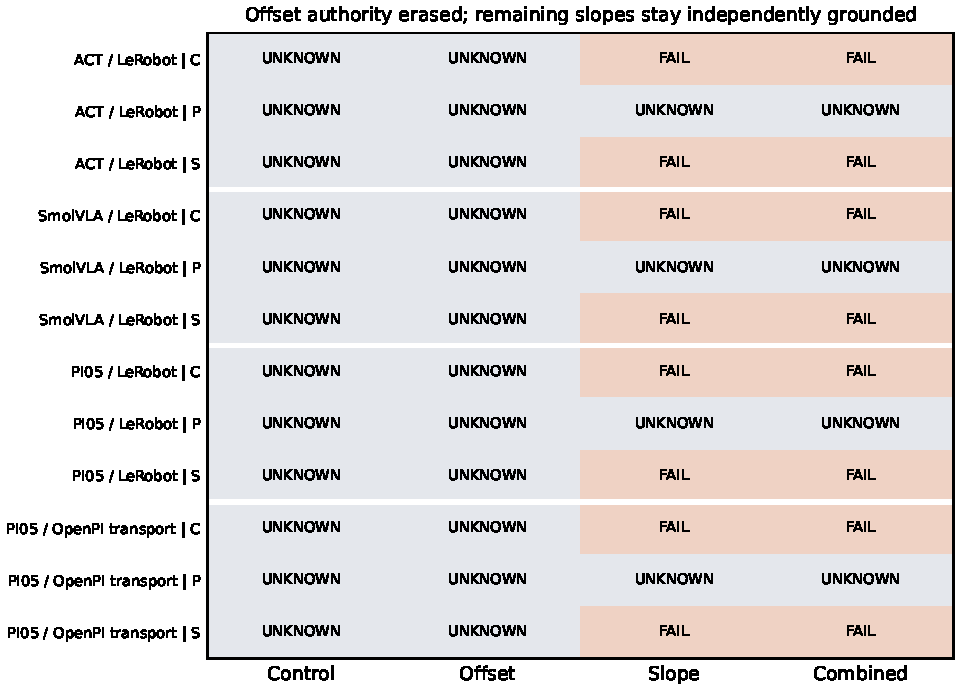
\includegraphics[width=\linewidth]{generated/authority-ablation.pdf}
\caption{Actual offset-authority ablations, grouped by execution cell. C: compiled; P: pointwise; S: strong relational. Cells, methods and interventions are repeated views, not independent samples. Remaining slope authority supports the two relational methods on the last two columns.}
\label{fig:authority}
\end{figure}

\subsection{Different contracts yield different correct outcomes}
Native APIs execute without asserting conformance. Candidate self round trips are within the frozen allowance for all sixteen actual conditions, including changed maps. An inverse pair can be internally consistent while implementing another numerical interface. Supplying an independent intended map to the round trip restores the distinction and matches the applicable numerical checks here.

Robotruth retains the known statistics-identity differences in the twelve changed deployments. Full executable-policy certification is withheld in every condition because required evidence is absent. This is neither sixteen fault detections nor four false alarms. Policy Space accepts all \MainPrimary{} structurally valid raw-vector replays and rejects sixteen separately designed structural controls. Acceptance answers transport validity, not numerical equality. The separately recorded float32 conversion also prevents a float64 decoder verdict from being silently attributed to the post-transport boundary. A development-only unchanged-value F64 serialization control further separates numerical agreement from strict artifact identity; it is not added to selected controls after evaluation.

\subsection{Fresh witnesses and cost}
Fresh processes reproduce each original failed relation. Figure~\ref{fig:witness} compares per-method retained views: the compiler requires \CompiledWitnessCalls{} native calls, versus \PointwiseWitnessCalls{} for pointwise and \StrongWitnessCalls{} for strong relational checks. The slope contrast uses two queries while an available absolute pointwise discrepancy uses one. Shared fresh acquisition costs \MainFresh{} calls because the views overlap. These results reject a witness-size improvement under this metric; no global minimality is claimed.

\begin{figure}[t]
\centering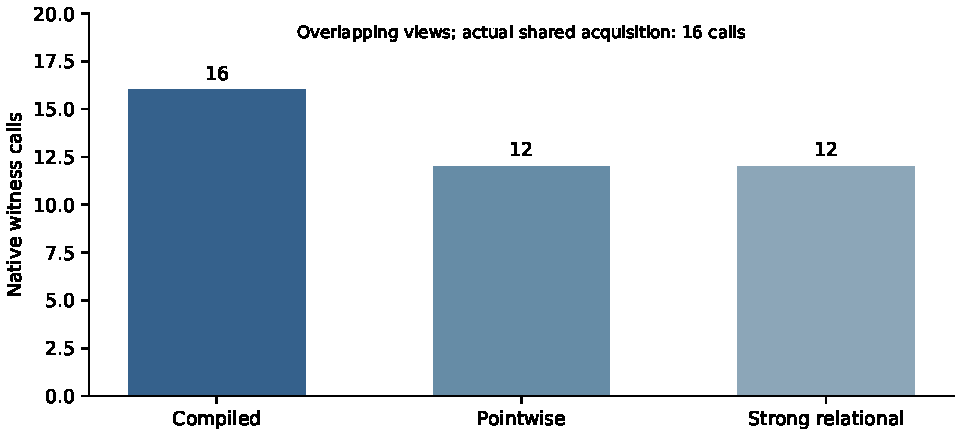
\includegraphics[width=.87\linewidth]{generated/witness-cost.pdf}
\caption{Total native calls in each method's fresh witness views over the fixed injected conditions. These overlapping views share sixteen actual acquisition calls. Call counts describe this artifact, not independent accuracy samples or human debugging time.}
\label{fig:witness}
\end{figure}

Original parent receipts total \ParentWall{} seconds of subprocess wall time, and measured native intervals total \NativeCPU{} process CPU seconds. Imports, initial gates and uncontrolled system/file caches matter; the two measures have different coverage and must not be subtracted to estimate a method's speed. The artifact reports setup/acquisition/evaluation fields, observed RSS and tracked implementation lines. Lines of code and executed commands are not measurements of human integration effort.

\subsection{Temporal and software-controller strata}
Two independently reproduced historical parent/fix incidents ground temporal/composition relevance: LeRobot PR4057's chunk-anchor behavior and OpenPI PR351's legacy data-factory convention. Their authority follows the documented training/deployment convention, rather than an assumed universally correct action representation. These are retrospective source-backed processor experiments, not selected newly discovered incidents or task evaluations.

On one reused scalar SO101 development cluster, the original stateful checker and compiler agree on eight matched conditions. Original prefix witnesses use 1--2 native actions, compared with 2--4 for the compiler. The original full report has extra first-action/queue/horizon checks; its runtime is not an equal-scope baseline. This reinforces the negative witness finding and prevents an action-only study from claiming temporal superiority.

A separate source-grounded Panda/robosuite stratum executes translation operators, full goal setters, noncommuting rotations, gripper integration and populated-state reset in an offline MuJoCo environment. Independent nonlinear/stateful references distinguish reversed rotation composition and omitted reset. The affine method retains \UNKNOWN{} on orientation and gripper lifecycle. Translation parity and a limited stateless subdomain illustrate the importance of observed state directions. A clean installation reproduces the semantic outputs. There are zero physics steps, torque calls or renders. This supplies a second software-embodiment stratum, not a mapping from PI checkpoint metadata to Panda hardware.

\section{Reproducibility, limitations and responsible use}
The artifact preserves raw arrays, exact loaded Safetensors identities/dtypes, all tool findings, requests/claims/receipts, source/package inventories, analysis and CSV output. Data-only replay regenerates the semantic products and checks the same committed freeze. The implementation passed 390 tests with five skips before freezing, including forty wrapper tests covering tampering beyond repaired digest chains, phase order, repeated requests and timeout-stream retention. Package installation and earlier controller/incident integrations have separate validation records.

Clean main reproduction requires four distinct separately installed environment directories with the same Python/package profiles and a verified original-summary hash. It compares semantic JSON/CSV products byte for byte and metrics with measured runtime fields excluded. Dependency setup failures are preserved separately: Windows Git long paths and an extra optional package in a broader install lock were repaired before the clean attempt, without changing the frozen distribution inventory or experimental methods. Fresh installations can reuse package caches and are on the same machine; this is not independent hardware replication. The achieved main clean result is \texttt{SEMANTIC\_ARTIFACTS\_REPRODUCED}: analysis, witness reports, joined workflow reports and the condition CSV reproduce byte for byte, and the finite metrics agree with measured phase costs excluded. The original and clean summary hashes and all six distinct native phase prefixes are recorded in the clean comparison file.

The strongest limitation is authority. Metadata-derived raw-index agreement is conditional on the supplied reference and current profile. It establishes neither calibrated units nor checkpoint-training identity. Correlated artifacts, few controls, known intervention recipes, outcome-unseen rather than blinded selection, and common reference mistakes constrain empirical reach. Binary64 probes do not characterize ordinary learned-output distributions or every deployment dtype. Framework imports include unused classes; full upstream training/inference dependency compatibility is not established by a processor subset. Non-affine operators and opaque callbacks require separate methods. Unsupported baselines remain limitations.

The practical lesson is to publish a verdict with its boundary and evidence requirements. A structural acceptance, an identity finding, an unknown physical mapping and a numerical failure can coexist without contradiction. Strong manual relational checks must be credited when automation matches them. Investigating genuine operator diversity and independently calibrated controller contracts is a future study, rather than an unreported extension of these counts.

\paragraph{Broader impact and authorship.}
These tools can support offline diagnosis and expose evidence gaps, but an unjustified physical \PASS{} could encourage unsafe deployment. The implementation keeps execution explicit, uses no live robot and withholds unsupported physical claims. Pinned public metadata and license declarations are preserved; no private data or weights are uploaded. This technical report has not been submitted to or accepted by a peer-reviewed venue.

\begin{samepage}
\paragraph{AI assistance disclosure.}
Artificial intelligence (AI) tools were used for manuscript editing and code preparation.
AI tools were used for research planning and experimental design; code preparation and testing; data analysis and interpretation; figure preparation; and manuscript drafting, revision, and review. The human author(s) retain responsibility for the final work. The automated checks and AI-assisted reviews reported here are not independent human peer review. Recorded assistance includes OpenAI Codex/ChatGPT tools during October 2026; exact model identifiers were not consistently recorded, and no model version is asserted.
\end{samepage}

\section{Conclusion}
This bounded study finds numerical parity among compiled obligations, strong independent checks and applicable static/reference workflows across pinned processor cells. Native self round trips, artifact certification and transport checks answer different questions, and missing physical authority survives numerical agreement. The compiler supplies replayable experiments and relation-preserving witnesses, but its witnesses are larger here and its affine scope is explicit. Reproducible evidence separation and honest negative findings are the contribution of this artifact; superior detection, policy performance and hardware safety remain unestablished.
